\chapter{Sistema de linealización, conversión coma flotante a coma fija y normalización}

En la implementación del circuito completo se utilizan dos etapas:

\begin{compactitem}

\item \nt{Corriente $i_{pv}$}: El bloque para la corriente requiere las etapas de linealización, conversión de la salida del linealizador de coma flotante a coma fija, y un normalizador con una salida de corriente entre el rango [-1,1].

\item \nt{Tensión $V_{pv}$}: La tensión del panel se trabaja de manera lineal, solo se requiere de un normalizador que contenga la salida de tensión entre el intervalo [0,1]. 

\end{compactitem}

\begin{figure}[H]
  \centering
    \includegraphics[scale=0.04]{./Linealizador_normalizador.png}
    \rule{35em}{0.5pt}
  \caption[Diseño general de entradas y salidas para el sistema  de linealización, conversión y normalización de corriente y tensión para un panel fotovoltaico]{Diseño general de entradas y salidas para el sistema  de linealización, conversión y normalización de corriente y tensión para un panel fotovoltaico.}
  \label{fig:Sist1}
\end{figure}


El sistema de la figura \ref{fig:Sist1} cuenta con 6 entradas y 4 salidas, estas se describen a continuación. 

Entradas:
\begin{compactitem}

\item \nt{CLK}: Reloj del sistema.
\item \nt{I}: Dato de corriente no lineal, en formato IEEE 754
\item \nt{V}: Dato de tensión en formato IEEE 754
\item \nt{RST\_LN\_FF}: Reset para las unidades de corriente y tensión. 
\item \nt{Begin\_FSM\_I}: Inicia la máquina de estados del linealizador de corriente. 
\item \nt{Begin\_FSM\_V}: Inicia la máquina de estados de el convertidor coma flotante-coma fija para la tensión. 

\end{compactitem}
Salidas:

\begin{compactitem}

\item \nt{ACK\_I}: Indica que el resultado de las operaciones para la corriente se encuentra listo.  
\item \nt{ACK\_V}: Indica que el resultado de las operaciones para la tensión se encuentra listo.  
\item \nt{RESULT\_I}: Resultado de corriente lineal y normalizado en formato coma fija. 
\item \nt{RESULT\_V}: Resultado de de tensión normalizado en formato coma fija.

\end{compactitem}

\begin{figure}[H]
  \centering
    \includegraphics[scale=0.05]{./Linealizador_normalizador2.png}
    \rule{35em}{0.5pt}
  \caption[Sistema de linealización, conversión y normalización de corriente y tensión para un panel fotovoltaico, con entradas: corriente $i_{pv}$ y tensión $V_{pv}$ y salidas de corriente y tensión lineales y normalizadas]{Sistema de linealización, conversión y normalización de corriente y tensión para un panel fotovoltaico, con entradas: corriente $i_{pv}$ y tensión $V_{pv}$ y salidas de corriente y tensión lineales y normalizadas}
  \label{fig:Sist2}
\end{figure}

La figura \ref{fig:Sist2} muestra la distribución de bloques funcionales sincronizados con un mismo reloj $ \left(CLK\right)$, para la corriente $i_{pv}$ y tensión $V_{pv}$ del panel fotovoltaico. Dentro de la sección de corriente se realiza primeramente la linealización, iniciando con las señales RST\_LN\_FF y Begin\_FSM\_I y el dato de entrada I (corriente $\ i_{pv}$), una vez ejecutada la operación se envía una señal indicando que el dato esta listo ACK\_LN; esta se conecta a la señal de entrada e inicio del convertidor-normalizador de corriente Begin\_FF. Un ciclo de reloj antes de que inicie la conversión-normalizacion, el resultado de la linealización $ \left(RESULT\right)$ esta listo, este resultado linealizado se conecta a la entrada F del convertidor-normalizador. La ejecución del resultado final linealizado y normalizado, se comprueba con la señal ACK\_I, esta indica que la conversión-normalización fue realizada y el resultado se encuentra en RESULT\_I (corriente lineal y normalizada en coma fija  $\ y' $).    

El bloque de tensión funciona de manera similar al de corriente, iniciando con las señales RST\_LN\_FF y Begin\_FSM\_V y el dato de entrada V (tensión $\ V_{pv}$). Una vez ejecutada la operación se envía una señal indicando que el dato esta listo ACK\_V y el resultado se despliega en RESULT\_V (tensión normalizada en coma fija  $\ z' $).

\section{Sistema para realizar las pruebas en una placa de desarrollo Nexys-4}

Para desarrollar las pruebas en la FPGA, se requirió diseñar e implementar un circuito para insertar datos a la entrada del linealizador-normalizador, sean procesados y posteriormente enviados por medio de transmisión serial hacia un computador.  

En la figura \ref{fig:flujo-test} se muestra el diagrama de flujo utilizado para realizar las pruebas de simulación y comprobación de los resultados experimentales del circuito completo. 

\begin{figure}[H]
  \centering
    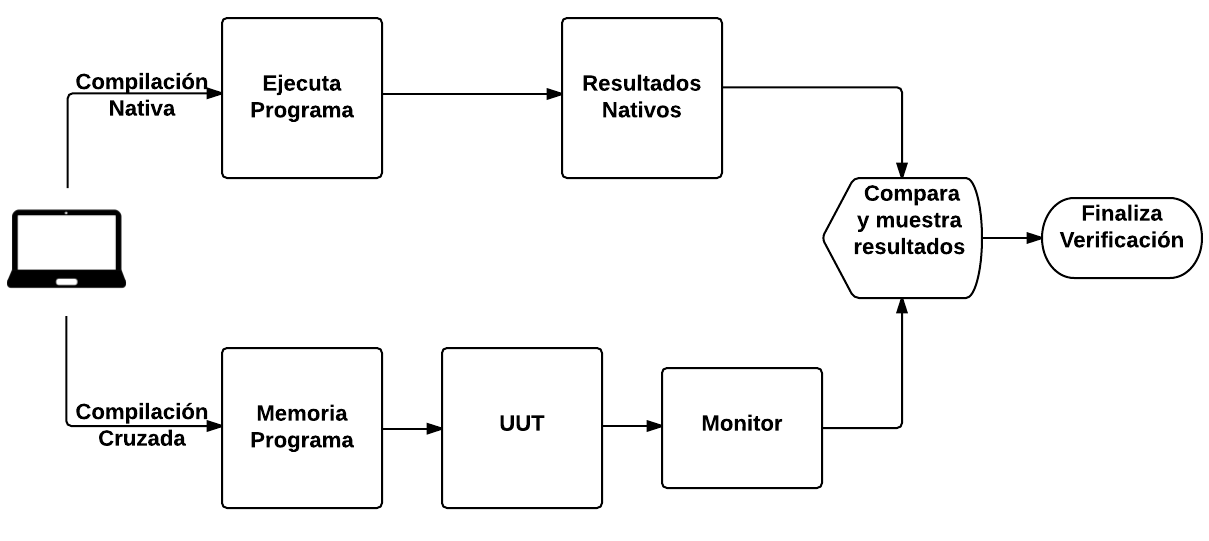
\includegraphics[scale=0.5]{./AmbienteVerificacion1.png}
    \rule{35em}{0.5pt}
  \caption[Diagrama de flujo general para el ambiente de verificación utilizado en el procesamiento de datos del circuito de linealización, ingresando los datos de entrada por medio de una memoria ROM y enviando los datos de salida por medio de transmisión serial (UART) desde la nexys-4 hacia un computador]{Diagrama de flujo general para el ambiente de verificación utilizado en el procesamiento de datos del circuito de linealización, ingresando los datos de entrada por medio de una memoria ROM y enviando los datos de salida por medio de transmisión serial (UART) desde la nexys-4 hacia un computador (Tomado de $ [15] $).}
  \label{fig:flujo-test}
\end{figure}


\begin{figure}[H]
  \centering
    \includegraphics[scale=0.06]{./test.png}
    \rule{35em}{0.5pt}
  \caption[Sistema de verificación para el linealizador, ingresando los datos de entrada por medio de una memoria ROM y enviando los datos de salida por medio de transmisión serial (UART) desde la nexys-4 hacia un computador]{Sistema de verificación para el linealizador, ingresando los datos de entrada por medio de una memoria ROM y enviando los datos de salida por medio de transmisión serial (UART) desde la nexys-4 hacia un computador}
  \label{fig:test}
\end{figure}

El diagrama de la figura \ref{fig:test} muestra el sistema utilizado. 
Primeramente se ingresan 1024 datos almacenados en una memoria ROM. Un archivo de texto contiene los datos de entrada para el linealizador-normalizador y se carga desde la memoria ROM. para direccionar esta memoria se cuenta do un contador de 10 bits. 
La sección de transmisión posee una unidad UART (transmisión serial), esta se utiliza para enviar los resultados de la unidad de linealización-normalización hacia el computador. Los resultados linealizados-noramlizados tienen un formato coma fija de 32 bits y el uart envía únicamente paquetes de 8 bits, por lo que se requiere enviar 4 paquetes por cada resultado, esto se logra por medio de una configuración de un multiplexor 4x1 y un contador; las entradas del multiplexor contienen el resultado dividido en paquetes de 8 bits, por medio del contador se selecciona el multiplexor según sea el paquete que se desea enviar. 
Por ultimo se cuenta con un control para el circuito, este se encarga de llevar la sincronía de los datos. Se realiza una carga en el contador de la memoria ROM, este direcciona la primera posición de la ROM y se inicia el procesamiento por parte de la unidad de linealización-normalización, con la señal $\ Begin\_op$; el control espera a que el resultado este listo por medio de la señal ACK. Cuando se da la condición ACK=High, el sistema se encuentra listo para transmitir, el contador del multiplexor selecciona el primer paquete y lo envía. El siguiente paquete se puede transmitir hasta que el modulo UART envié de vuelta al control, la señal $\ TX\_DONE$, así sucesivamente hasta que se envíen los 4 paquetes. Cuando la selección del multiplexor esta en 2b'11 (contador del multiplexor), la señal $\ max\_tick\_mux$ indica al control que debe realizar una cuenta para la dirección de la ROM y asi tomar el siguiente dato a procesar. 
Este proceso se repite hasta que la cuenta de las direcciones de la ROM es 1023 y la señal $\ max\_tick\_add = 1 $.
La recepción de datos desde el computador se realizó por medio de un puerto USB y un "script" realizado en Matlab. Este recibe los paquetes de un byte en hexadecimal y los concatena en paquetes de 4 bytes, para formar el dato en 32 bits, posteriormente se convierte a decimal.   


\section{Simulación del sistema de linealización, conversión coma flotante a coma fija y normalización, implementado en hardware mediante verilog}

Este circuito se implementó por medio de la unión de los bloques anteriormente diseñados, implementados y simulados. 

Para esta comprobacion se utilizaron 1000 valores que describen el comportamiento real de un PV, utilizando el modelo del panel.  Este toma un valor de tensión $ V_{pv} $ para cada valor de tiempo a partir de la ecuación \ref{eq:ej4}, y se sustituye en la ecuación \ref{eq:ej5} obteniendo valores de corriente de entrada $ i_{pv} $ para el linealizador. 

\begin{equation} \label{eq:ej4}
   V_{pv} = V_{cte} + 0.3*V_{cte}*sin(2* \pi *100*t)     
\end{equation}

    
\begin{equation} \label{eq:ej5}
   i_{pv} = Ig - \frac{V_{pv}}{R_p} - Is*\left(e^\frac{V_{pv}* \alpha}{2}\right)         
\end{equation} 

 

\begin{figure}[H]
  \centering
    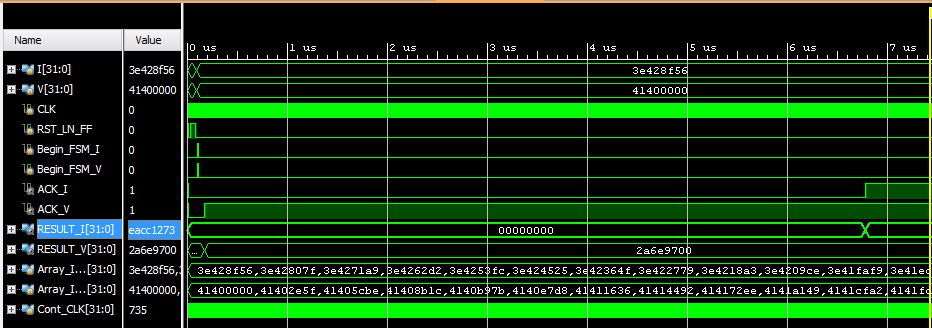
\includegraphics[scale=0.6]{./TEST_LINEALIZADOR_NORMALIZADOR.png}
    \rule{35em}{0.5pt}
  \caption[Simulación del sistema de linealización-conversión-normalización de corriente y sistema de conversión- normalización de tensión para un panel fotovoltaico]{Simulación del sistema de linealización-conversión-normalización de corriente y sistema de conversión- normalización de tensión para un panel fotovoltaico}
  \label{fig:Sim_Sist}
\end{figure}
\newpage
La simulación básica "behavioral" efectuada por Vivado, verifica el funcionamiento adecuado del circuito a manera de software y de lógica sin embargo no es suficiente ya que se debe realizar la sintesis e implementación, para esto se realizan las simulaciones post-syntesis y post-implementation, tanto del funcionamiento como de los retardos del sistema. La figura \ref{fig:Sim_Sist} muestra la simulación de tiempos posterior a la implementación, utilizado los valores de entrada de tensión y corriente a partir del modelo del panel.

\section{Resultados del sistema de linealización, conversión coma flotante a coma fija y normalización implementado en una placa de desarrollo nexys-4}

Las simulaciones para el circuito completo brindan una mejor información acerca del porcentaje de error total obtenido dentro de la conexión de las tres etapas  linealización, conversión y normalización. Se efectuaron las simulaciones de temporización y funcionalidad posterior a la síntesis, obteniendo resultados experimentales para realizar una comparación contra los teóricos esperados.      
 
En el capítulo 3 se demostró el funcionamiento del linealizador con 8,12 y 15 iteraciones para el rango de convergencia del algoritmo de CORDIC, en este capítulo se utiliza el mismo principio de verificación, sin embargo se debe contemplar el error del normalizador, por lo que se realizan pruebas y comparaciones similares utilizando como datos de entrada un barrido de 1000 valores ingresados en el modelo teórico del panel fotovoltaico, esto con el fin de observar un comportamiento similar al real. Los valores de corriente son pequeños debido a la diferencia de corrientes y perdidas en el panel fotovoltaico, por lo que los porcentajes de error serán menores debido a que el circuito posee una mejor aproximación; en el extremo inferior del intervalo de convergencia del algoritmo CORDIC. 
La visualización de los resultados obtenidos se realiza de una mejor manera mediante gráficos que indican como se comporta el circuito ante datos de entrada, salida, y porcentaje de error. A partir de los resultados de las simulaciones, se puede analizar la frecuencia de ejecución a la que se obtiene un resultado linealizado-normalizado, esta depende del número de iteraciones que se utilice.
El tiempo de ejecución de la unidad completa, contempla los ciclos de cada uno de los bloques funcionales que componen la ruta de ejecución de la corriente este circuito.
Si tomamos el bloque para la tensión, este solo cuenta con la conversión-normalización y no depende del número de iteraciones por lo que se requieren de 8 ciclos de reloj por cada dato. 

\newpage

\begin{table}[H]
\centering
\caption{Comparación de resultados experimentales obtenidos por del sistema de verificación implementado en una placa de desarrollo nexys-4, a partir de los valores de entrada del del modelo del panel y utilizando 8, 12 y 15 iteraciones en el algoritmo de CORDIC. CLK=100MHz. }
\label{Table:comparacion_iter}
\begin{tabular}{|c|c|c|c|c|c|c|}
\hline
$  $ & 8 iteraciones  & 12 iteraciones  & 15 iteraciones      \\ \hline


\begin{tabular}[c]{@{}c@{}} Error máximo (\%)
\end{tabular}  & 0,922 & 0,259   & 0,129         \\ \hline

\begin{tabular}[c]{@{}c@{}} Error promedio (\%)
\end{tabular}  & 0,455 & 0,0351   & 0,0257        \\ \hline

\begin{tabular}[c]{@{}c@{}} Desviación estándar 
\end{tabular} & 0,2695 & 0,0253   & 0,0082     \\ \hline

\begin{tabular}[c]{@{}c@{}} Número de ciclos 
\end{tabular}  & 468 & 668   & 826        \\ \hline

\begin{tabular}[c]{@{}c@{}} Frecuencia de ejecución (kHz) 
\end{tabular} & 217 & 151   & 121       \\ \hline

\begin{tabular}[c]{@{}l@{}} Tiempo de ejecución ($ \mu s$)
\end{tabular} & 4,68 & 6,68   & 8,26      \\ \hline


\end{tabular}
\end{table}


Utilizando 8 iteraciones en el algoritmo de CORDIC y a partir de las simulaciones post-síntesis efectuadas por medio de la herramienta Vivado, se requiere de 468 ciclos de reloj para completar la ejecución de un dato, este se compone de 460 ciclos de reloj para el linealizador y 8 ciclos de reloj para el convertidor-normalizador, donde la velocidad de ejecución es de 4,68$ \mu s$ (217kHz) con un reloj de sistema de 100MHz.  

\begin{figure}[H]
  \centering
    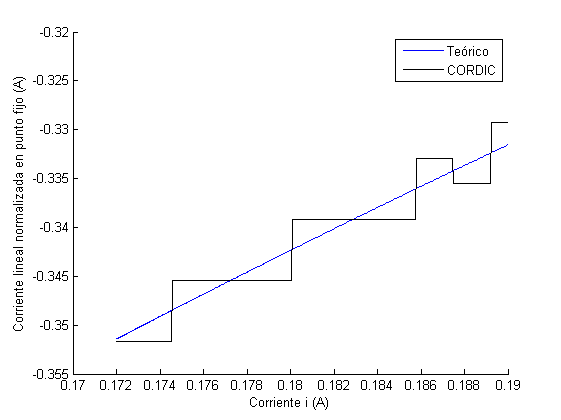
\includegraphics[scale=0.8]{./LINEALIZADOR_NORMALIZADOR_8iter.png}
    \rule{35em}{0.5pt}
  \caption[Comparación entre el valor teórico y el valor obtenido del circuito de linealización-conversión-normalización de corriente con 8 iteraciones en el algoritmo de CORDIC del linealizador]{Comparación entre el valor teórico y el valor obtenido del circuito de linealización-conversión-normalización de corriente con 8 iteraciones en el algoritmo de CORDIC del linealizador}
  \label{fig:LIN_NOR_8}
\end{figure}

\newpage 

\begin{figure}[H]
  \centering
    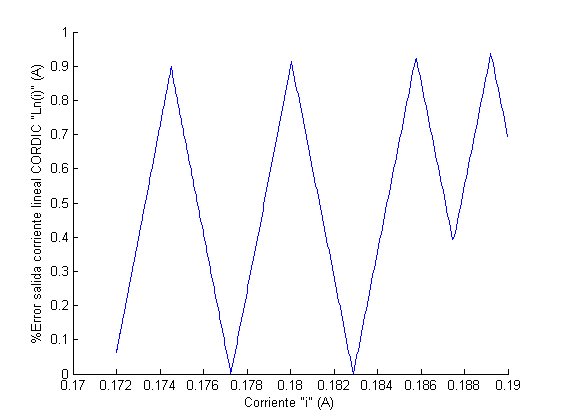
\includegraphics[scale=0.8]{./LINEALIZADOR_NORMALIZADOR_8iter_ERROR.png}
    \rule{35em}{0.5pt}
  \caption[Porcentaje de error entre el valor teórico y el valor obtenido del circuito de linealización-conversión-normalización de corriente con 8 iteraciones en el algoritmo de CORDIC del linealizador]{Porcentaje de error entre el valor teórico y el valor obtenido del circuito de linealización-conversión-normalización de corriente con 8 iteraciones en el algoritmo de CORDIC del linealizador}
  \label{fig:LIN_NOR_8_E}
\end{figure}

En la figura \ref{fig:LIN_NOR_8} se puede observar la comparación entre los datos obtenidos del circuito implementado en una placa nexys-4, contra los datos teóricos al realizar la misma función del circuito. Debido a que son solo 8 iteraciones el circuito posee un resultados aceptables pero poco exactos. El gráfico muestra que el algoritmo trata de mantenerse cerca de los valores reales, sin embargo posee un comportamiento escalonado, en donde para cierta cantidad de valores de entrada posee un mismo valor de salida constante cercano al valor real. 

La figura \ref{fig:LIN_NOR_8_E} muestra el porcentaje de error asociado a cada valor de entrada linealizado y normalizado en formato coma fija, donde el porcentaje de error máximo es de 0,922\% y un porcentaje de error promedio de 0,455\% y una desviación estándar de 0,2695, esto para valores de corriente derivados a partir del modelo teórico del panel fotovoltaico. 
  

Utilizando 12 iteraciones en el algoritmo de CORDIC, se requiere de 668 ciclos de reloj para realizar el procesamiento completo de un dato de entrada, 660 ciclos de reloj son utilizados por el linealizador y 8 ciclos de reloj para el convertidor-normalizador. Este se ejecuta con una velocidad de 6.68$ \mu s$ (151kHz), utilizando un reloj de sistema de 100MHz.   

\newpage
\begin{figure}[H]
  \centering
    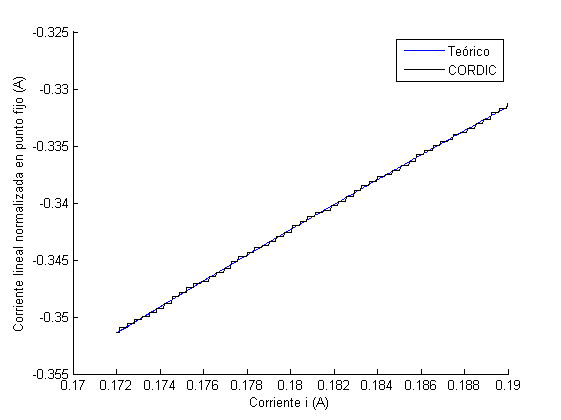
\includegraphics[scale=0.8]{./LINEALIZADOR_NORMALIZADOR_12iter.png}
    \rule{35em}{0.5pt}
  \caption[Comparación entre el valor teórico y el valor obtenido del circuito de linealización-conversión-normalización de corriente con 12 iteraciones en el algoritmo de CORDIC del linealizador]{Comparación entre el valor teórico y el valor obtenido del circuito de linealización-conversión-normalización de corriente con 12 iteraciones en el algoritmo de CORDIC del linealizador}
  \label{fig:LIN_NOR_12}
\end{figure}


\begin{figure}[H]
  \centering
    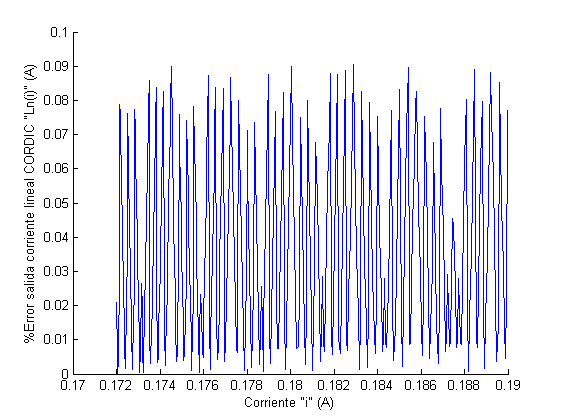
\includegraphics[scale=0.8]{./LINEALIZADOR_NORMALIZADOR_12iter_ERROR.png}
    \rule{35em}{0.5pt}
  \caption[Porcentaje de error entre el valor teórico y el valor obtenido del circuito de linealización-conversión-normalización de corriente con 12 iteraciones en el algoritmo de CORDIC del linealizador]{Porcentaje de error entre el valor teórico y el valor obtenido del circuito de linealización-conversión-normalización de corriente con 12 iteraciones en el algoritmo de CORDIC del linealizador}
  \label{fig:LIN_NOR_12_E}
\end{figure}

En la figura \ref{fig:LIN_NOR_12} se puede observar la comparación entre los datos obtenidos experimentalmente contra los datos teóricos al realizar la misma función del circuito utilizando 12 iteraciones. Brinda una mejor exactitud contra 8 iteraciones y se puede observar que presenta una mayor suavidad en la curva, sin embargo presenta un comportamiento escalonado pero con un valores más cercanos a la curva real. 
La figura \ref{fig:LIN_NOR_12_E} muestra el porcentaje de error asociado a cada valor de entrada linealizado con 12 iteraciones y normalizado en formato coma fija. Donde el porcentaje de error máximo es de 0,0897\% y un porcentaje de error promedio de 0,0345\% y una desviación estándar de 0,0253, esto para valores de corriente derivados a partir del modelo teórico del panel fotovoltaico.

En el sistema del panel es de suma importancia el tiempo de muestreo según sea la frecuencia del panel, esto implica velocidad de ejecución dentro del cálculo. Se logró determinar que con 15 iteraciones se obtienen resultados con muy buena exactitud,sin embargo el tiempo de ejecución aumenta a 826 ciclos de reloj, tomando en cuenta que 818 ciclos son requeridos por el linealizador y 8 ciclos de reloj para la conversión de formato IEEE 754 a coma fija y normalización. Donde la velocidad de ejecución es de 8.26$ \mu s$ (121kHz) con un reloj de sistema de 100MHz.  


\begin{figure}[H]
  \centering
    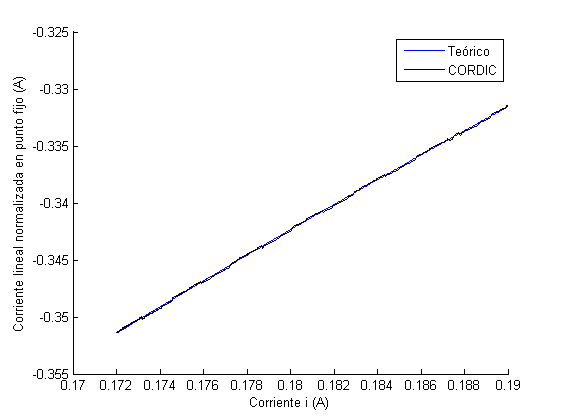
\includegraphics[scale=0.8]{./LINEALIZADOR_NORMALIZADOR_15iter.png}
    \rule{35em}{0.5pt}
  \caption[Comparación entre el valor teórico y el valor obtenido del circuito de linealización-conversión-normalización de corriente con 15 iteraciones en el algoritmo de CORDIC del linealizador]{Comparación entre el valor teórico y el valor obtenido del circuito de linealización-conversión-normalización de corriente con 15 iteraciones en el algoritmo de CORDIC del linealizador}
  \label{fig:LIN_NOR_15}
\end{figure}

\begin{figure}[H]
  \centering
    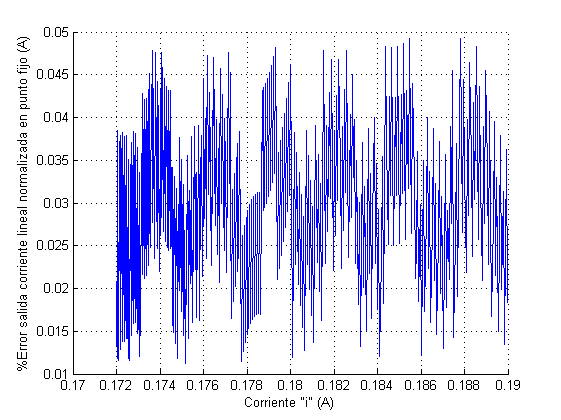
\includegraphics[scale=0.8]{./LINEALIZADOR_NORMALIZADOR_15iter_ERROR.png}
    \rule{35em}{0.5pt}
  \caption[Porcentaje de error entre el valor teórico y el valor obtenido del circuito de linealización-conversión-normalización de corriente con 15 iteraciones en el algoritmo de CORDIC del linealizador]{Porcentaje de error entre el valor teórico y el valor obtenido del circuito de linealización-conversión-normalización de corriente con 15 iteraciones en el algoritmo de CORDIC del linealizador}
  \label{fig:LIN_NOR_15_E}
\end{figure}

Con 15 iteraciones el valor experimental es muy similar al valor teórico, como se observa en la figura \ref{fig:LIN_NOR_15}, y se puede comprobar en la figura \ref{fig:LIN_NOR_15_E} donde se muestra que el porcentaje de error es muy cercano a cero, con un valor máximo de 0,0483\% y un error promedio de 0,0292\% y una desviación estándar de 0,0082, esto para valores de corriente derivados a partir del modelo teórico del panel fotovoltaico.

El sistema de optimización se utilizará en un panel fotovoltaico que posee una frecuencia de 100kHz, es decir que el sistema de optimización debe realizar un cálculo completo a una velocidad mayor que el panel. Aproximadamente el sistema de linealización y normalización toma un 40\% del total del tiempo de ejecución del sistema de optimización, por lo que se requiere realizar el cálculo en el tiempo indicado, para esto se deberá utilizar 8 iteraciones.    

\newpage 

\section{Recursos utilizados}


\begin{table}[H]
\centering
\caption{Resumen del reporte post implementación del uso de dispositivos generado por la herramienta Vivado.}
\label{Table:Recursos}
\begin{tabular}{|c|c|c|c|c|c|}
\hline
Recurso & Utilizados  & Disponibles & Utilizados\%   \\ \hline

\begin{tabular}[c]{@{}c@{}} LUT
\end{tabular}  & 1017 &  63400   & 1.60      \\ \hline

\begin{tabular}[c]{@{}c@{}} FF
\end{tabular} & 912 & 126800   & 0.72         \\ \hline

\begin{tabular}[c]{@{}c@{}} DSP 
\end{tabular} & 4 & 240   & 1.67       \\ \hline

\begin{tabular}[c]{@{}l@{}} IO
\end{tabular} & 134 & 210   & 63.81     \\ \hline

\begin{tabular}[c]{@{}l@{}} BUFG
\end{tabular} & 1 & 32   & 3.12   \\ \hline

\end{tabular}
\end{table}

En la tabla \ref{Table:Recursos} se muestra el uso de recursos para la implementación el circuito completo en la Nexys4, el máximo recurso utilizado son los puertos I/O debido a que se requieren 32 bits en cada entrada I,V y 32 bits en cada salida RESULT\_I , RESULT\_V, sin embargo el uso de los demás recursos es sumamente bajo, el uso de los I/O se reducirá debido a que este circuito se deben acoplar a otro bloques del sistema de optimización.
  
\section{Reporte de tiempos}

Dentro del reporte de tiempos se analizan las peores rutas "ruta critica", para un buen diseño se requiere de un slack positivo. El mayor slack del circuito linealizador-normalizador es de 4.5 lo que indica que los datos llegan a tiempo, con este slack se puede aproximar que el circuito puede funcionar a una frecuencia de 200MHz.    

\section{Consumo de potencia}
Con la ayuda de las herramientas de análisis de potencia de Vivado, se pudo obtener los resultados que pertenecen al consumo de potencia, tanto estática como dinámica. En la tabla \ref{Table:Potencia1} se muestra el valor para cada consumo, y el total. 

\begin{table}[H]
\centering
\caption{Resumen del reporte post implementación de la potencia estática, dinámica y total, de la herramienta Vivado, para el sistema de linealización-normalización.}
\label{Table:Potencia1}
\begin{tabular}{|c|c|c|}
\hline
Potencia  & Consumo de potencia $ \left(mW\right) $      \\ \hline

\begin{tabular}[c]{@{}c@{}} Dinámica
\end{tabular}  & 11         \\ \hline

\begin{tabular}[c]{@{}c@{}} Estática
\end{tabular}  & 91          \\ \hline

\begin{tabular}[c]{@{}c@{}} Total
\end{tabular}  & 102         \\ \hline



\end{tabular}
\end{table}


Para los recursos utilizados se puede realizar un estudio de consumo de potencia dinámica, estos resultados se muestran en la tabla \ref{Table:Potencia2} donde el mayor consumo de potencia se presenta por parte del reloj del sistema y señales, las señales que poseen un valor de cero no se refieren a un consumo nulo, si no que es relativamente pequeño en comparación con las señales mas criticas.

\begin{table}[H]
\centering
\caption{Resumen del reporte generado por la herramienta Vivado que indica el consumo de potencia de diversos elementos. }
\label{Table:Potencia2}
\begin{tabular}{|c|c|c|c|c|c|c|}
\hline
On-chip $ \left(mW\right)$ & Consumo de potencia $ \left(mW\right) $      \\ \hline

\begin{tabular}[c]{@{}c@{}} Clocks
\end{tabular}  & 4          \\ \hline

\begin{tabular}[c]{@{}c@{}} Signals
\end{tabular}  & 4          \\ \hline

\begin{tabular}[c]{@{}c@{}} Logic
\end{tabular}  & 3          \\ \hline

\begin{tabular}[c]{@{}c@{}} DSP
\end{tabular}  & 0          \\ \hline

\begin{tabular}[c]{@{}c@{}} I/O
\end{tabular}  & 0          \\ \hline


\end{tabular}
\end{table}







